%! TEX root = ./main.tex

\section{Application Layer}
\begin{itemize}
    \item Top-most layer
    \item Used by user-applications as well as core internet applications
\end{itemize}

\subsection{Domain Name Service (DNS)}
\begin{itemize}
    \item Provides core functionality for the internet
    \item Human identify hosts using hostnames, while internet uses IPs
    \item DNS provides hostnames to IP mapping
    \item It is not one-to-one mapping:
        \begin{itemize}
            \ides{Load Balancing:} One hostname maps to multiple IP
            \ides{Reuse hardware:} Multiple hostnames map to same IP
                \begin{itemize}
                    \item E.g. host multiple websites on same machine
                \end{itemize}
        \end{itemize}
    \ides{History}
        \begin{itemize}
            \item One list of all mappings
            \item Manually shared and updated
            \item Placed in \verb+/etc/hosts+
            \icon Not scalable
            \icon Hard to manage
            \icon Inconsistent
            \icon List no always available for download
        \end{itemize}
    \ipro Scalability
    \ipro Availability
        \begin{itemize}
            \item Domains are independent of each other
        \end{itemize}
    \ipro Extensible
        \begin{itemize}
            \item Can extend any part without interference of other parts
        \end{itemize}
\end{itemize}

\subsubsection{Structure}
\begin{itemize}
    \item DNS uses three intertwined hierarchies
        \begin{itemize}
            \ides{Naming Structure}
                \begin{itemize}
                    \ides{Root:}
                        \begin{itemize}
                            \item Imaginary dot after the TLD in the URL
                        \end{itemize}
                    \ides{Top Level Domain (TLD):} Sit at the top
                    \ides{Domain:} Subtree of the TLD
                    \ides{Subdomain:} Subtree of domain
                        \begin{itemize}
                            \item Can be arbitrarily nested
                        \end{itemize}
                    \item A name is a leaf-to-root path
                \end{itemize}
            \ides{Management}
                \begin{itemize}
                    \item Root is managed by the IANA
                        \begin{itemize}
                            \item Association of 13 companies
                        \end{itemize}
                    \item TLDs are managed by private or federal organisations
                    \item Domains are managed by private organisations
                        \begin{itemize}
                            \item I.e. Hosting companies and ISPs
                        \end{itemize}
                    \ipro Name collision is trivially avoided
                \end{itemize}
            \ides{Infrastructure}
                \begin{itemize}
                    \item $13$ root servers
                        \begin{itemize}
                            \item Named \textit{a} through \textit{m}
                            \item Each has numerous mirrors
                            \item Distributed all around the world
                            \item Two \textit{k} root server are located in CH
                        \end{itemize}
                    \item TLD are managed professionally
                    \item Domains are managed by ISPs or locally
                \end{itemize}
        \end{itemize}
    \ides{BGP Anycast}
        \begin{itemize}
            \item Allows sharing of same IP for multiple servers
            \item Determines ``fastest'' path
                \begin{itemize}
                    \item Not necessarily the shortest
                \end{itemize}
            \item Used by the roots servers for load balancing
            \item Allows DNS system to scale
        \end{itemize}
    \item For the system to work, we need
        \begin{itemize}
            \item Each DNS server knows the address of the root server
            \item Each root servers knows the address of all TLD servers
            \item Each DNS server knows the address of all its children
        \end{itemize}
    \ides{DNS Server}
        \begin{itemize}
            \item Each domain must have at least two DNS server
                \begin{itemize}
                    \item Ensure availability
                    \item Load-balancing
                \end{itemize}
            \item Stores \textit{Resource Records} as tuples \verb+(name, value, type, TTL)+
                \begin{itemize}
                    \ides{Name:} The variable which we want to map
                    \ides{Value:} Desired value
                    \ides{Type:} One of:

                        \begin{tabular}{l l l}
                            Record Type & Name & Value\\
                            \hline
                            A & hostname & IP address\\
                            NS & domain & DNS server name\\
                            MX & domain & Mail server name\\
                            CNAME & alias & canonical name\\
                            PTR & IP address & corresponding hostname
                        \end{tabular}
                    \ides{Time-to-Life (TTL):} How long the mapping is valid
                        \begin{itemize}
                            \item Used for caching
                        \end{itemize}
                \end{itemize}
        \end{itemize}
\end{itemize}

\subsubsection{DNS Query}
\begin{itemize}
    \item Used UDP on port 53
        \begin{itemize}
            \item Unreliable; may not get an answer
        \end{itemize}
    \ides{Main Steps}
        \begin{itemize}
            \item Browser wants to access a domain name
            \item OS triggers resolution process by sending request to local DNS server
            \item DNS systems translates domain
        \end{itemize}
    \ides{Local DNS Server}
        \begin{itemize}
            \item Normally closed to the endhost
            \item Can be either:
                \begin{itemize}
                    \ides{Locally:} Running on host
                    \ides{Enterprise:} Somewhere in the network
                    \ides{ISP:} Running by the ISP
                    \ides{External:} Run by a third-party company
                        \begin{itemize}
                            \icon Wrong geographical local
                            \icon PGB Anycast does not give fastest server
                            \icon Insecure
                        \end{itemize}
                \end{itemize}
            \item Endhosts can choose a DNS server by:
                \begin{itemize}
                    \item Hardcoding it to \verb+/etc/resolv.conf+
                    \item Rely on dynamic allocation by \verb+DHCP+
                \end{itemize}
        \end{itemize}
    \ides{Query Type}
        \begin{itemize}
            \ides{Recursive Query}
                \begin{itemize}
                    \item Client offloads task of resolving to the next server
                    \item Not done in practice
                        \begin{itemize}
                            \item Except for external resolvers apparently
                        \end{itemize}
                    \item Steps:
                        \begin{itemize}
                            \item DNS client asks DNS server for domain IP
                            \item DNS server queries root server
                            \item Root server queries TLD server
                            \item TLD server queries domain server
                            \item Domain server returns domain IP to TLD server
                            \item TLD server returns domain IP to root server
                            \item Root server returns domain IP to DNS server
                            \item DNS server return domain IP to DNS client
                        \end{itemize}
                    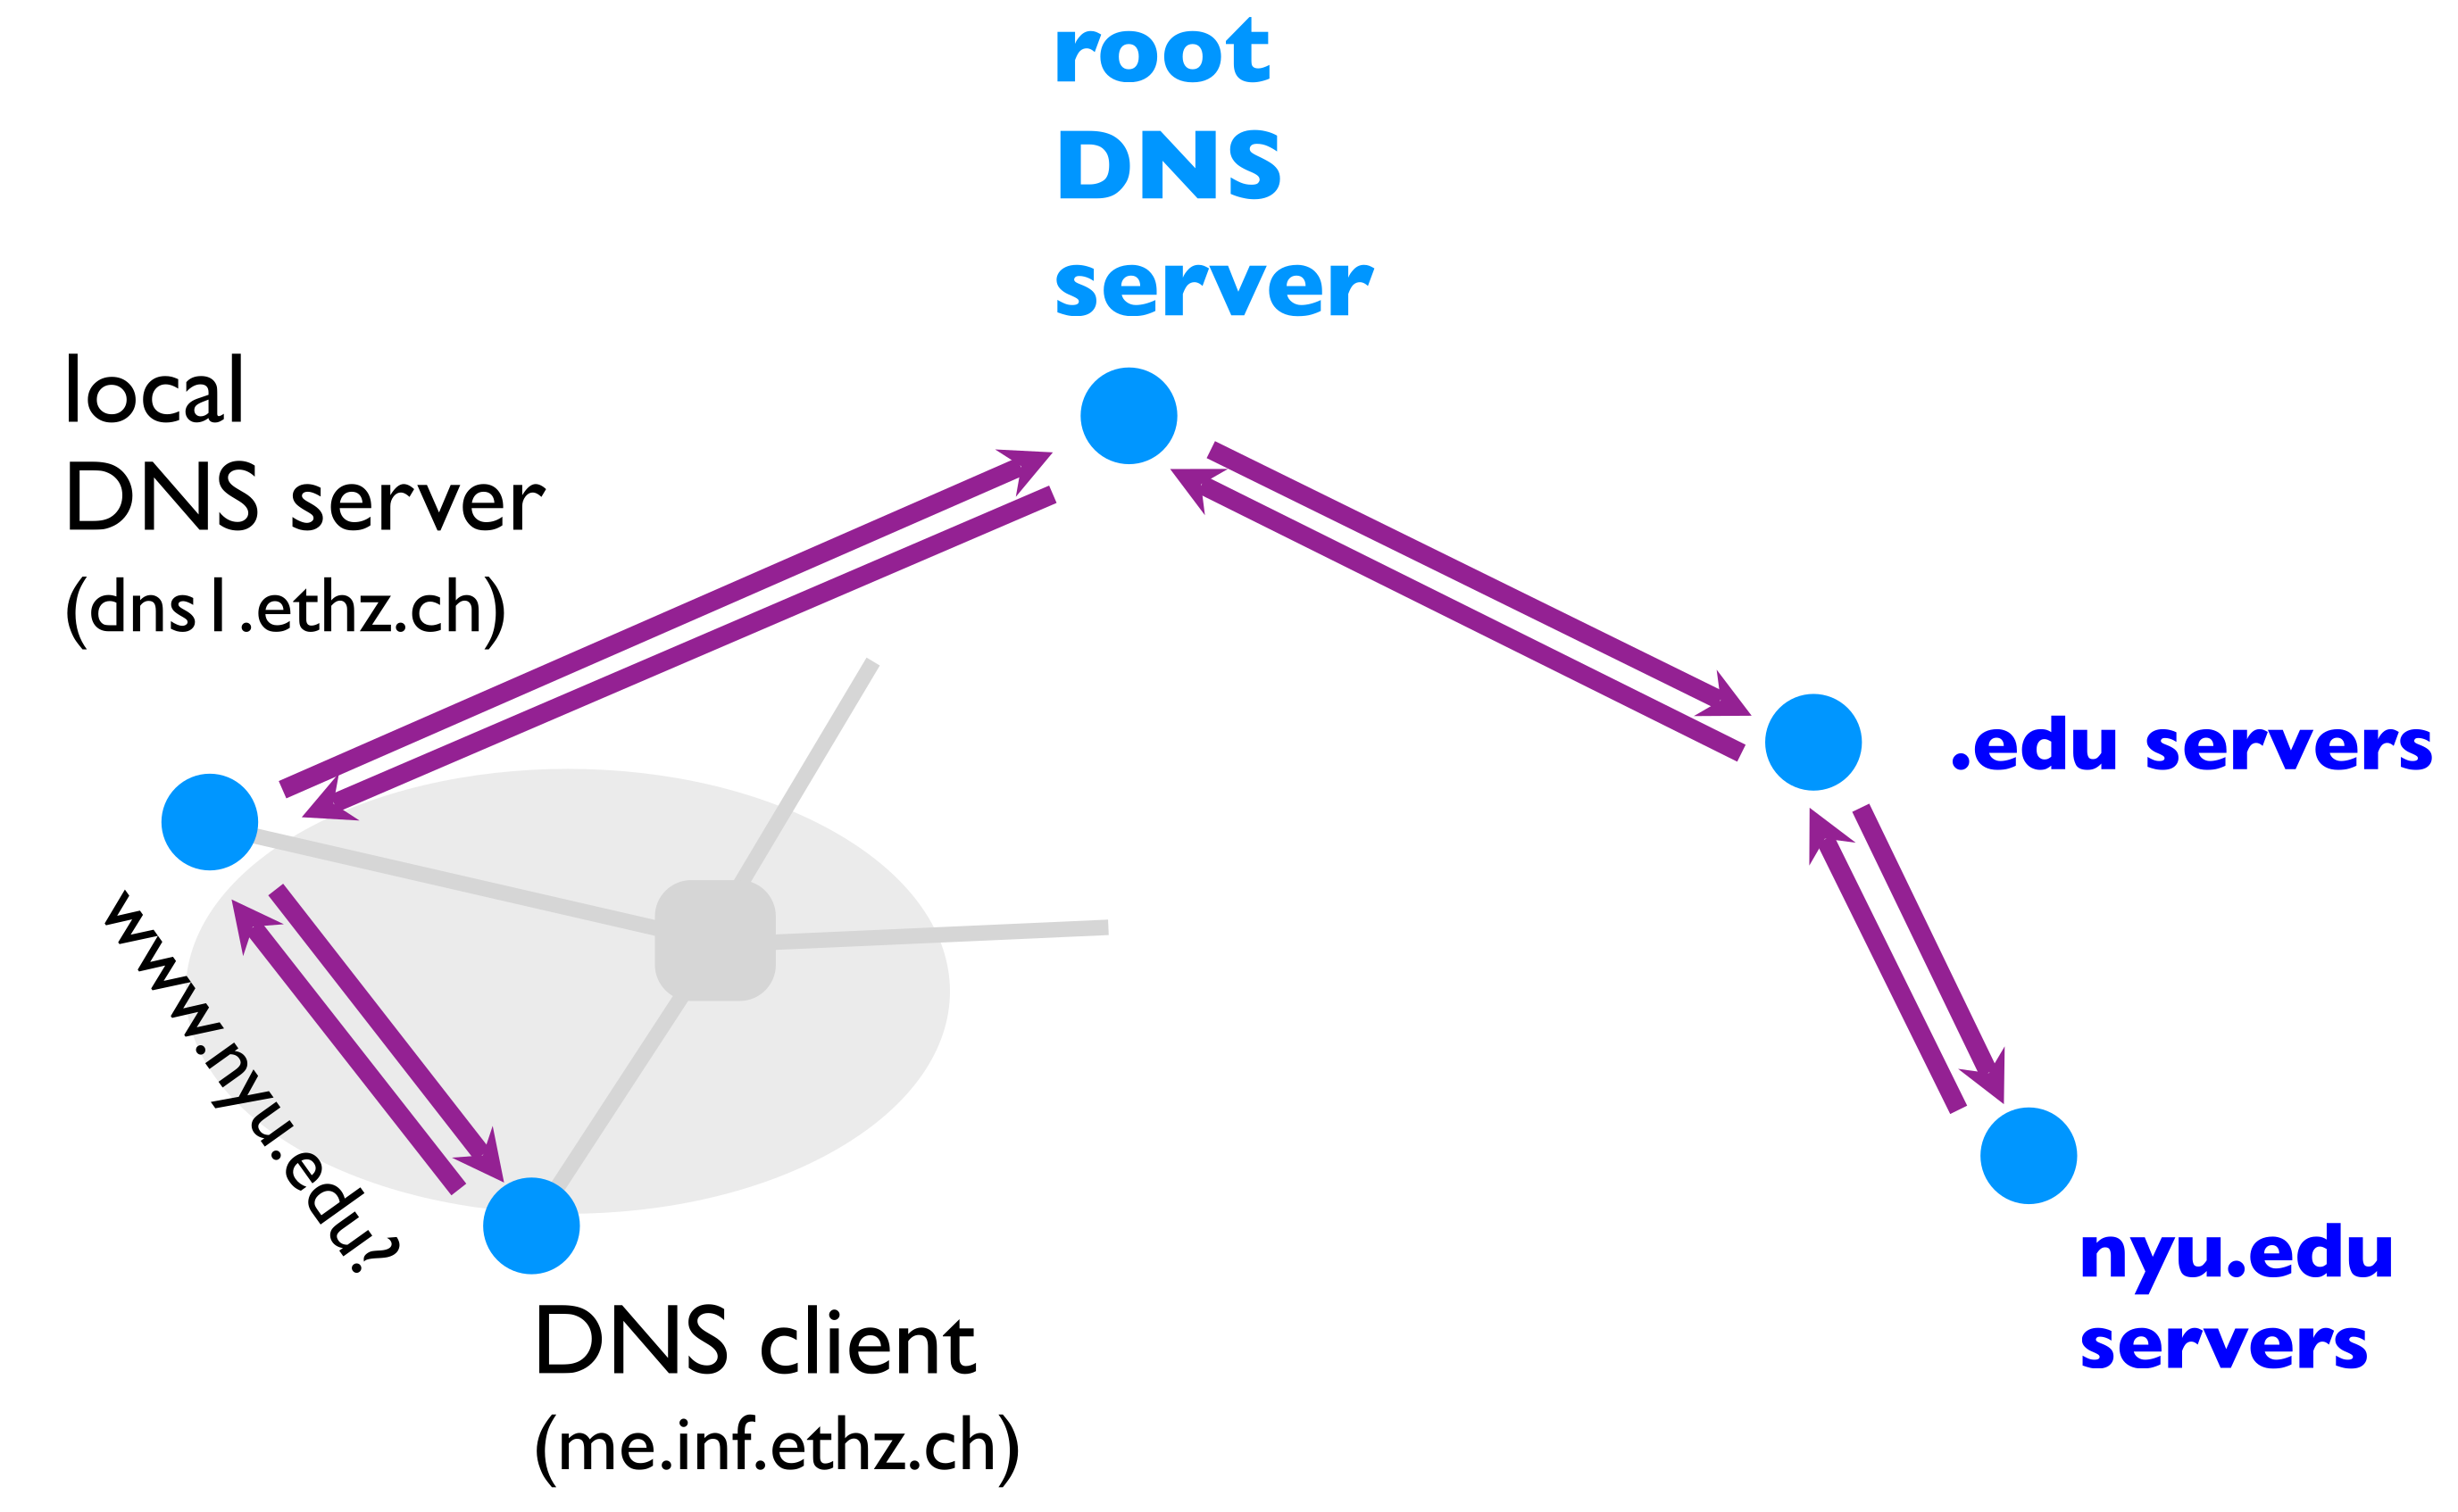
\includegraphics[width=0.8\textwidth]{dns_recursivequery.png}
                \end{itemize}
            \ides{Iterative Query}
                \begin{itemize}
                    \item Each server only returns address to next server
                    \item Steps
                        \begin{itemize}
                            \item DNS client asks DNS server for IP
                            \item DNS server queries root server
                            \item Root server returns TLD server IP to DNS server
                            \item DNS server queries TLD server at given IP
                            \item TLD server returns domain server IP to DNS server
                            \item DNS server queries domain server at given IP
                            \item Domain server returns domain IP to DNS server
                            \item DNS server return IP to DNS client
                        \end{itemize}
                    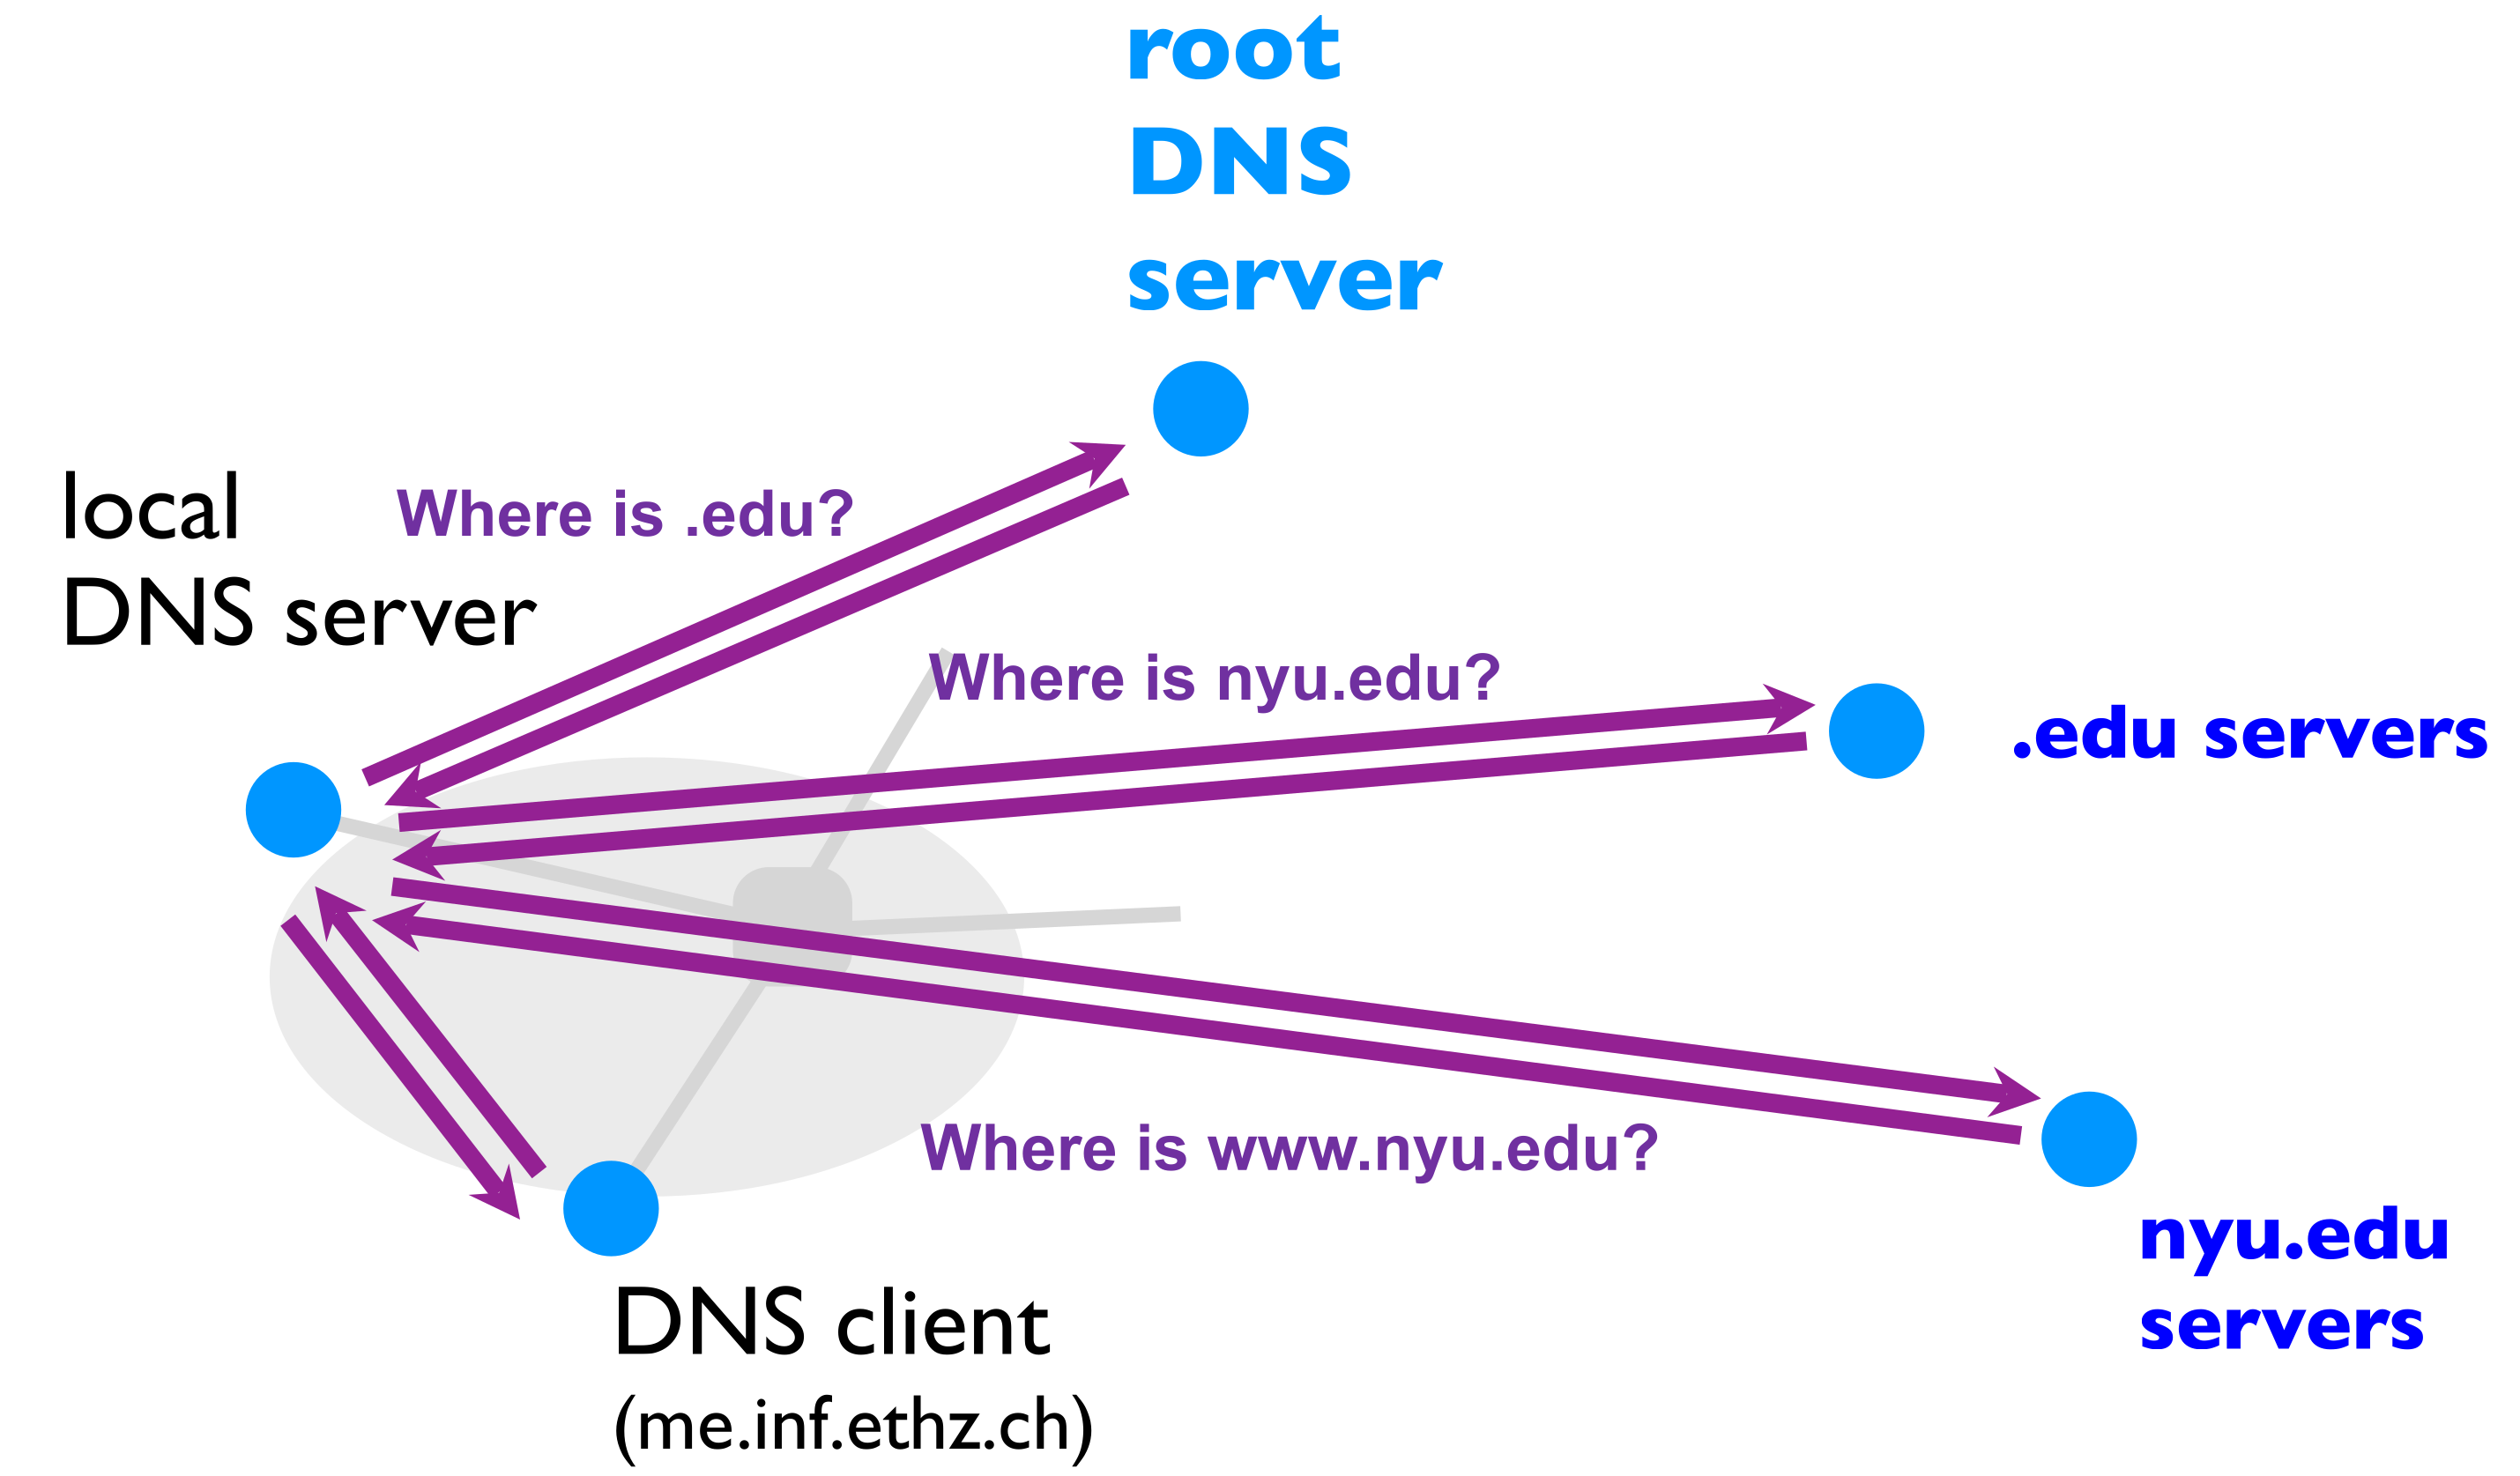
\includegraphics[width=0.8\textwidth]{dns_iterativequery.png}
                    \item Somehow we sometimes say that CNS client is recursively (makes only one request) while the DNS server is iteratively (makes many requests)
                \end{itemize}
        \end{itemize}
\end{itemize}

\subsubsection{Caching}
\begin{itemize}
    \item Most DNS queries requests the same site
    \item Cache result of former queries
    \item DNS records is cached for TTL seconds
    \item Hit rate of about $75\%$
\end{itemize}

\subsubsection{Problems}
\begin{itemize}
    \icon DNS is vital for the internet
        \begin{itemize}
            \item Server not accessible when DNS server not available
        \end{itemize}
    \icon DNS servers can see the sites one visits
        \begin{itemize}
            \item Sell data
        \end{itemize}
    \icon Vulnerable to different security breaches
\end{itemize}

\subsection{Web}
\begin{itemize}
    \item Distributed database of pages
    \item Composed of:
        \begin{itemize}
            \ides{Infrastructure:} Client/Browser, servers, proxies
            \ides{Content:} Objects organized in web sites
            \ides{Implementation:} URL, HTTP
        \end{itemize}
\end{itemize}

\subsubsection{URL}
\begin{itemize}
    \ides{Uniform Resource Locator (URL):} address to a internet source
    \item \verb+protocol://hostname[:port]/directory_path/resource+
        \begin{itemize}
            \ides{Protocol:} e.g. HTTP(S), FTP, SMTP etc.
            \ides{Hostname:} DNS name or IP address
            \ides{Port:} Optional and defaults to protocol standard
                \begin{itemize}
                    \item $80$ for HTTP, $443$ for HTTPS
                \end{itemize}
                \ides{Directory\_path/Resource:} Identify resource on destination
        \end{itemize}
\end{itemize}

\subsubsection{HTTP}
\begin{itemize}
    \ides{Hypertext Transfer Protocol (HTTP)}
    \ipro Simple
    \item Properties
        \begin{itemize}
            \item Synchronous Request-Response: make request and wait
            \item Layered over a bidirectional byte stream: Build on TCP (most of the times)
            \item Text-Based: Human readable
            \item State-Less: No info about past client requests
        \end{itemize}
    \ides{Request}
        \begin{itemize}
            \item Message is composed of header and body
            \item Following three header fields are required
            \ides{Method:}
                \begin{itemize}
                    \ides{GET:} request resource
                    \ides{HEAD:} request headers only
                        \begin{itemize}
                            \item E.g. used by bots
                        \end{itemize}
                    \ides{POST:} send data to the server
                \end{itemize}
            \ides{URL:} Relative (to server) address of resource
            \ides{Version:} HTTP version to use
            \item Can have many other optional header fields
                \begin{itemize}
                    \item Header has a variable length
                \end{itemize}
        \end{itemize}
    \ides{Response}
        \begin{itemize}
            \item Message is composed of header and body
            \item Following three header fields are required
            \ides{Version:} HTTP version to use
            \ides{Status:} Status code
                \begin{itemize}
                    \ides{1XX:} Informational
                    \ides{2XX:} Success
                    \ides{3XX:} Redirection
                    \ides{4XX:} Client Error
                    \ides{5XX:} Server Error
                \end{itemize}
            \ides{Phrase:} Status message
                \begin{itemize}
                    \item Associated with status code
                \end{itemize}
            \item Can have many other optional header fields
                \begin{itemize}
                    \item Header has a variable length
                \end{itemize}
        \end{itemize}
    \ides{Cookies}
        \begin{itemize}
            \ides{Stateless:} Each request is treated independently
                \begin{itemize}
                    \ipro Server-side scalability
                    \ipro Failure handling is trivial
                    \icon Some application need state
                \end{itemize}
            \ides{Cookie:} Small textfile saved on the client side
                \begin{itemize}
                    \item Sent along with each request
                    \item Server can request us to update the content
                \end{itemize}
        \end{itemize}
    \ides{Web Page}
        \begin{itemize}
            \item Web pages consist of man different resources
            \item All resources have to be fetched
            \item Resources have to be compile according to their dependency
                \begin{itemize}
                    \item Prevent race conditions
                    \item Browser has to be conservative
                    \item Model as DAG
                        \begin{itemize}
                            \ides{Node:} Task (fetch or compile)
                            \ides{Edge:} Must-happen-before Relationship
                            \ides{Weight:} Time predeceasing task takes
                        \end{itemize}
                    \item Loading time is equal the critical path (the longest path) length
                    \item Find using either algorithm:
                        \begin{itemize}
                            \item Top-Sort
                            \item Recursively find the longest path for each node
                        \end{itemize}
                    \item Costs $O(n + v)$
                    \item Speed-up task on critical path will shorten or change the critical path
                \end{itemize}
            \item Loading time is ambiguously defined
                \begin{itemize}
                    \item I.e. not clear when page has finished loading
                \end{itemize}
        \end{itemize}
    \ides{Speed-up}
        \begin{itemize}
            \item Many techniques to speed-up the loading
            \ides{Simplify and Restructure Web Page}
                \begin{itemize}
                    \item Prevent cross dependency
                    \item Better compression
                    \item Inline code
                    \item Mark resources as asynchronous
                        \ides{Minify:} Make code as compact as possible
                \end{itemize}
            \ides{Faster End-Devices}
                \begin{itemize}
                    \item Shorter rendering time
                \end{itemize}
            \ides{Better Network Infrastructure}
                \begin{itemize}
                    \item Decrease fetching time
                    \item Diminishing Returns
                \end{itemize}
            \ides{Decrease RTT}
                \begin{itemize}
                    \item Great improvement
                    \item Hard to achieve in practice
                \end{itemize}
            \ides{Simplify Network Protocols}
                \begin{itemize}
                    \item Naive HTTP opens one TCP connection per object
                        \begin{itemize}
                            \item Fetch $n$ objects costs $2n$ RTT
                        \end{itemize}
                    \item Use $M$ parallel connection
                        \begin{itemize}
                            \item Fetch $n$ objects costs $2n / M$ RTT
                            \icon Burden to server
                            \icon Bandwidth contention
                        \end{itemize}
                    \item Use persistent connection
                        \begin{itemize}
                            \item Fetch $n$ objects costs $n + 1$ RTT
                            \item Default in HTTP/1.1
                            \ipro Reduce connection setup and tear down cost
                            \ipro Allow for more accurate RTT estimation
                            \ipro Allow TCP congestion window to increase
                        \end{itemize}
                    \item Use parallel requests/responses
                        \begin{itemize}
                            \item Fetch $n$ objects costs $2$ RTT
                                \begin{itemize}
                                    \item Assume that the packets are not too large
                                \end{itemize}
                            \item Pack multiple requests into one large
                        \end{itemize}
                \end{itemize}
            \ides{Caching}
                \begin{itemize}
                    \item Same, unchanged resources are fetched over and over
                    \ipro Saves time
                    \ipro Decreases server load
                    \ipro Decreases network load
                    \item Significant portion of objects are uncachable
                        \begin{itemize}
                            \item Dynamic data (e.g. weather)
                            \item Scripts (where the result depends on some parameters)
                            \item Cookies (result may depend on sent cookie)
                            \item SSL encrypted content
                            \item Advertising
                        \end{itemize}
                    \item Clients send in the request the time they have last fetched the object. The server sends the object only when it was changed in the mean time.
                    \item Caches are at:
                        \begin{itemize}
                            \ides{Client:} Browser Cache
                            \ides{Close to Client:} By ISP, CDN or enterprise network
                            \ides{Close to Destination:} Reverse proxy
                        \end{itemize}
                \end{itemize}
            \ides{Replication}
                \begin{itemize}
                    \item See CDN section below
                \end{itemize}
        \end{itemize}
\end{itemize}

\subsection{Internet Video}
\begin{itemize}
    \item Requirement: Good quality without rebuffering
    \item Different viewers have different setups and therefore have different requirements
    \ides{End-End Workflow:}
        \begin{itemize}
            \item Encode video in multiple qualities and resolutions
                \begin{itemize}
                    \item Resulting in encodings of different bitrate
                \end{itemize}
            \item Replicate content using CDN
            \item Player picks appropriate quality
                \begin{itemize}
                    \item Manifest file gives information about available bitrates
                    \item Clients can pick different qualities for different chunks
                        \begin{itemize}
                            \item Each chunk is about $1$ to $3$ seconds long
                        \end{itemize}
                    \ides{Capacity Estimation:} Estimate bandwidth and choose video with smaller bitrate than estimated bandwidth
                    \ides{Buffer-Based Adaption:} Choose bitrate based on buffered duration
                        \begin{itemize}
                            \item Need to differentiate startup phase
                        \end{itemize}
                    \item Both algorithms can be combined
                \end{itemize}
        \end{itemize}
    \ides{Bitrate} of a video is the size of video divided by the length of the video

\end{itemize}

\subsection{Content Delivery Network / Content Distribution Network (CDN)}
\begin{itemize}
    \item Not an application itself but used by web and video
    \item Spread popular content among data centres around the world
    \item Interconnect CDN server
    \item Direct clients to CDN instead of original server
        \begin{itemize}
            \item Done using either:
                \begin{itemize}
                    \ides{DNS-Based}
                        \begin{itemize}
                            \item Returns different IP addresses for same domain
                            \item Based on geo-location
                            \item Requires rewriting of URL in the source files
                            \icon May not result in good experience when using external DNS resolvers
                        \end{itemize}
                    \ides{BGP Anycast}
                        \begin{itemize}
                            \item Always give same IP
                            \item BGP directs traffic to ``closest'' CDN server
                            \ipro Easy
                            \icon Less flexible
                            \icon Less control
                        \end{itemize}
                \end{itemize}
        \end{itemize}
    \item Two types of caching:
        \begin{itemize}
            \ides{Pull Caching:} Cache whatever clients request
            \ides{Pull Replication:} Cache popular content before user request it
        \end{itemize}
    \ipro Load balancing
    \ipro Better reliability
        \begin{itemize}
            \item No single source of failure
        \end{itemize}
    \ipro Content is closer to the client
        \begin{itemize}
            \item Reduce latency
        \end{itemize}
    \ipro Speedup uncachable data
\end{itemize}
